% Generated by plsimcount.pfseeds -- do not edit; regenerate instead.
% figure: A-measured-by-order -- Suzuki formulas of each order, r from: Measured $r$; median over seeds [1, 2, 3, 4, 5], bars = min..max
% metric=t gatebase=ct merged
% seed 1: git_commit=04cd66abb614bdc66fb48e891cef085a299e0ab1 git_dirty=False
% seed 2: git_commit=04cd66abb614bdc66fb48e891cef085a299e0ab1 git_dirty=False
% seed 3: git_commit=04cd66abb614bdc66fb48e891cef085a299e0ab1 git_dirty=False
% seed 4: git_commit=04cd66abb614bdc66fb48e891cef085a299e0ab1 git_dirty=False
% seed 5: git_commit=04cd66abb614bdc66fb48e891cef085a299e0ab1 git_dirty=False
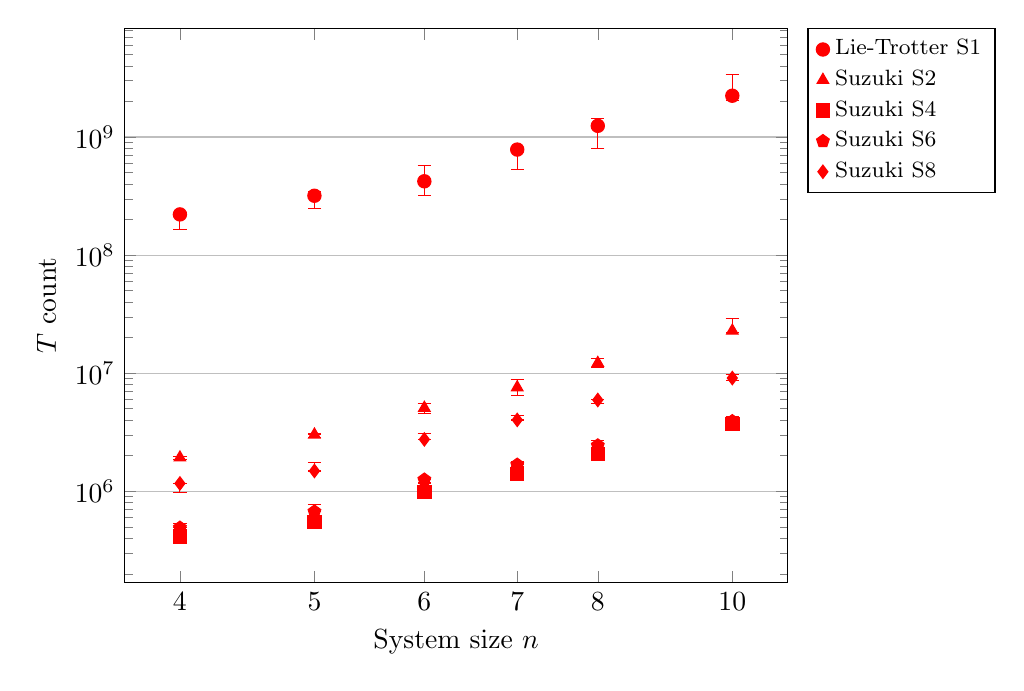
\begin{tikzpicture}
  \begin{loglogaxis}[
    width=10cm,
    xlabel={System size $n$},
    ylabel={$T$ count},
    xtick={4,5,6,7,8,10},
    xticklabels={4,5,6,7,8,10},
    ymajorgrids=true,
    legend pos=outer north east,
    legend cell align=left,
    legend style={font=\footnotesize},
  ]
    \addplot[only marks, red, mark=*, mark size=2.4pt, mark options={solid, fill=red}, error bars/.cd, y dir=both, y explicit, error bar style={red}] coordinates {
      (4,221263504) += (0,9069896) -= (0,57191984)
      (5,318348120) += (0,25613720) -= (0,71149566)
      (6,422071546) += (0,150465926) -= (0,104463980)
      (7,783651672) += (0,13465684) -= (0,255736656)
      (8,1244572288) += (0,196329224) -= (0,447938996)
      (10,2238616720) += (0,1152727882) -= (0,211682584)
    };
    \addlegendentry{Lie-Trotter S1}
    \addplot[only marks, red, mark=triangle*, mark size=2.4pt, mark options={solid, fill=red}, error bars/.cd, y dir=both, y explicit, error bar style={red}] coordinates {
      (4,1927848) += (0,51480) -= (0,62594)
      (5,3015896) += (0,41928) -= (0,159878)
      (6,5084160) += (0,449116) -= (0,552112)
      (7,7580986) += (0,1287530) -= (0,1106698)
      (8,12184250) += (0,1241932) -= (0,912938)
      (10,22892562) += (0,6036462) -= (0,613252)
    };
    \addlegendentry{Suzuki S2}
    \addplot[only marks, red, mark=square*, mark size=2.4pt, mark options={solid, fill=red}, error bars/.cd, y dir=both, y explicit, error bar style={red}] coordinates {
      (4,413718) += (0,5272) -= (0,742)
      (5,547344) += (0,73710) -= (0,24870)
      (6,983882) += (0,33568) -= (0,66258)
      (7,1405320) += (0,220920) -= (0,90456)
      (8,2071296) += (0,126240) -= (0,50016)
      (10,3700064) += (0,450366) -= (0,118640)
    };
    \addlegendentry{Suzuki S4}
    \addplot[only marks, red, mark=pentagon*, mark size=2.4pt, mark options={solid, fill=red}, error bars/.cd, y dir=both, y explicit, error bar style={red}] coordinates {
      (4,490724) += (0,40968) -= (0,520)
      (5,672420) += (0,98108) -= (0,896)
      (6,1253994) += (0,1680) -= (0,79154)
      (7,1677264) += (0,122664) -= (0,4896)
      (8,2442300) += (0,271290) -= (0,100376)
      (10,3919472) += (0,396598) -= (0,115280)
    };
    \addlegendentry{Suzuki S6}
    \addplot[only marks, red, mark=diamond*, mark size=2.4pt, mark options={solid, fill=red}, error bars/.cd, y dir=both, y explicit, error bar style={red}] coordinates {
      (4,1164480) += (0,4188) -= (0,187970)
      (5,1485780) += (0,263786) -= (0,2340)
      (6,2749626) += (0,314354) -= (0,4482)
      (7,4021776) += (0,362808) -= (0,4268)
      (8,5928020) += (0,9996) -= (0,415968)
      (10,9094694) += (0,574114) -= (0,479014)
    };
    \addlegendentry{Suzuki S8}
  \end{loglogaxis}
\end{tikzpicture}
